% !TEX root=../pldi2019.tex



\section{Semantics}
\label{sec:semantics}

In this section we formalise the semantics of the language constructs described in \cref{sec:language}.
We organize this by following the structure of the language.

Firstly, the task language is embedded in a simply typed lambda calculus.
This requires a specification of the evaluation of terms in the host language, and how it handles the task language.

Secondly, there are two ways to drive evaluation of task expressions, internally by the system itself, and externally by the user.
This is done in two additional semantics, one for the internal normalisation of tasks, and another for the interaction with the end user.

One of our explicit goals is to keep the semantics for evaluation and normalization separate.
This is achieved by letting tasks be values in the host language.

The three main layers of semantics are thus \emph{evaluation}, \emph{normalisation}, and \emph{interaction}.
The semantics, together with \emph{observations}, will be discussed in the following subsections.
\Cref{fig:semantic-functions} shows the relation between the semantics.
It also shows that there are two helper semantics, \emph{handle} and \emph{stride}.

\begin{figure}[h]
  \centering
  \includegraphics[width=\columnwidth,page=5]{figures/drawings-crop.pdf}
  \caption{
    Semantic functions defined in this report and their relation.
  }
  \label{fig:semantic-functions}
\end{figure}

We use the convention that downward arrows are big-step semantics, and rightward arrows are small-step semantics.



\subsection{Evaluating expressions}
\label{sec:evaluation}

The host language evaluates expressions using a big-step semantics.
Evaluating an expression $e$ in state $s$ into a value $v$ in state $s'$ is denoted by $\RelationE$.
To ease reasoning about references, we choose a call-by-value evaluation strategy.

\Cref{fig:value-grammar} shows values with respect to the evaluation semantics.
Tasks are values, and the operands of task constructors are evaluated eagerly.
Exceptions to this are steps and external choice, where some or all of the operands are not evaluated.

\begin{figure}[h]
  \small
  \usemacro{G-Values-Compact}
  \caption{Value grammar} \label{fig:value-grammar}
\end{figure}

The rules to evaluate expressions $e$ do not differ from standard work, except for the task constructs.
The evaluation rules for tasks can be deduced from the value grammar.
They are given in the appendix.


\subsection{Task observations}

The normalisation and interaction semantics make use of observations on tasks.
Observations are semantic functions on the syntax tree of tasks.
There are four semantic functions: $\Value$ for the current task value, $\Failing$ to determine if a task fails, $\Inputs$ for the currently accepted input events, and a function for generating user interfaces.
The semantics make use of $\Value$ and $\Failing$, while $\Inputs$ is used for proving safety.
The function for user interfaces is not used by the semantics, but by our implementation.
It is only described in passing here.




\paragraph{Observable values $(\Value)$}

Task values are used by steps to calculate the successor task.
Filled editors are tasks which contain values, as are shared editors.
Unvalued editors do not contain values, neither does the fail task.
These facts propagate through all other task constructors.
The partial function $\Value$ associates a value $v$ to tasks $t$ where possible.
Its definition is given in \cref{fig:observation-value}.

\begin{figure}[h]
  \small
  \usemacro{O-Value}
  \caption{Values} \label{fig:observation-value}
\end{figure}

Internal and external steps do not have an observable value, because calculating the value would require evaluation of the continuation.
Parallel composition only has a value when both branches have values, in which case these values are paired.
Internal choice has a value when one of the branches has a value.
When both branches have a value, it takes the value of the left branch.
External choice does not have a value because it waits for user input.



\paragraph{Failing $(\Failing)$}

In \cref{sub:fail} we introduced $\Fail$ to stand for an impossible task.
Combinations of tasks can also be impossible.
Take for example the parallel composition of two fails ($\Fail \And \Fail$).
This expression is equivalent to $\Fail$, because it can not handle input and can not be further normalized.

This intuition is formalised by the function $\Failing$ in \cref{fig:observation-failing}.
It determines whether a task is impossible.
Such tasks are called \emph{failing}.

\begin{figure}[h]
  \small
  \usemacro{O-Failing}
  \caption{Failing} \label{fig:observation-failing}
\end{figure}

Steps whose left hand sides are failing can never proceed because of the lack of an observable value.
Therefore they are itself failing.
The internal choice of two failing tasks is failing.
External choices let the user pick a side and only then evaluate the corresponding subexpression.
To determine if an external choice is failing, it needs to peek into the future to check if both subexpressions are failing.
Annotations are failing only if the inner task is failing.



\paragraph{User interface}

\TOPHAT is designed such that a user interface can be generated from a task's syntax tree.
A possible graphical user interface is shown in \cref{fig:flight-booking}, where tasks are rendered as \HTML pages.
Editors are rendered as input fields,
external choices are represented by two buttons,
and parallel tasks are rendered side by side.
Steps only show the interface of their left hand side.
In case of an external step they are accompanied by a button.
When the guard condition of a step is not fulfilled, the button is disabled.



\subsection{Normalising tasks}
\label{sec:normalise}

Normalisation prepares tasks to handle any given input by the end user.
It is a big-step semantics which makes use of evaluation of the underlying host language.
We write $\RelationN$ to describe that
an expression $e$ in state $s$ normalises to task $t$ in state $s'$.
It is a semantic relation that acts on the task level
and only accepts expressions of type $\Task \tau$.

Normalisation rules are given in \cref{fig:normalisation-semantics}.
Both rules ensure expressions $e$ are first evaluated by the host language ($\evaluate$).
Then it will delegate work to the stride semantics ($\stride$) we will discuss below.
These two actions are repeated by \refrule{N-Repeat} till the resulting state and task stabilise,
which is expressed by \refrule{N-Done}.

\begin{figure}[h]
  \small

  \boxed{\RelationN}
  \begin{mathpar}
    \userule{N-Done} \\
    \userule{N-Repeat}
  \end{mathpar}
  \caption{Normalisation semantics} \label{fig:normalisation-semantics}

\end{figure}

The reason to split out striding from normalisation have to do with state.
% This would be quite straight-forward, if we did not have to deal with state.
Consider the following example
\begin{TASK}
  (update l >>= \x:Bool. if x then e else fail) <&> (l := True; edit <<>>)
\end{TASK}
with $s=\set{l\mapsto\False}$.
When we apply \refrule{S-And} in order to normalise the expression above, we obtain
\begin{TASK}
  (update l >>= \x:Bool. if x then e else fail) <&> (edit <<>>)
\end{TASK}
with $s'=\set{l\mapsto\True}$.
This expression in fact is not normalised.
The issue here lies in the fact that $s$ gets updated by the second component,
which allows the first component of $\And$ to be further normalised, in this case to $e$.
To overcome this problem, the \refrule{N-Done} and \refrule{N-Repeat} rules have been added.
They ensure that normalisation is applied until the shared memory $s$ has become stable and no further normalisation can be applied.

Striding semantics are intended to perform internal steps and internal choices.
A stride from task $t$ in state $s$ to $t'$ in state $s'$ is denoted by $\RelationS$.
All rules are given in \cref{fig:striding-semantics}.
Tasks like editors, fail and external choice are ready and stride to themselves.
For external choice, parallel, and appoint,
there are congruence rules.

\begin{figure}[h]
  \small

  \begin{mathpar}
    \boxed{\RelationS}
  \end{mathpar}

  \paragraph{Step}
  \begin{mathpar}
    \userule{S-ThenStay} \\
    \userule{S-ThenFail} \\
    \userule{S-ThenCont}
  \end{mathpar}

  \paragraph{Choose}
  \begin{mathpar}
    \userule{S-OrLeft} \\
    \userule{S-OrRight} \\
    \userule{S-OrNone}
  \end{mathpar}

  \paragraph{Ready}
  \begin{mathpar}
    \userule{S-Edit} \quad \userule{S-Fill} \qquad \userule{S-Update} \\
    \userule{S-Fail} \quad \userule{S-Xor}
  \end{mathpar}

  \paragraph{Congruence}
  \begin{mathpar}
    \userule{S-Next} \quad
    \userule{S-And} \\
    %\userule{S-Appoint}
    % \userule{S-Eval}
  \end{mathpar}

  \caption{Striding semantics} \label{fig:striding-semantics}
\end{figure}



\paragraph{Principles of stepping}
\label{sub:stepping-principles}

Stepping from task $t_1$ to its continuation $t_2$ can only be performed when
$t_1$ has an observable value ($\Value(t_1) = v_1$).
This uses the fact that that calculating a new task $t_2$ from an expression $e$
is not possible when there is no observable value of $t_1$ to pass on.
To protect users from stepping to a failing task,
we add the condition that $t_2$ is not failing ($\Failing(t_2) = \False$).

These principles lead to the step rules in \cref{fig:striding-semantics}.
\refrule{S-ThenStay} does nothing,
because the lhs does not have a value.
In the rule \refrule{S-ThenFail},
the lhs has a value, but the calculate continuation is failing.
Note it uses the semantics of the host language to evaluate the function application $e_2 v_1$.
In case the continuation is not failing,
\refrule{S-ThenCont} strides to this new task.



\paragraph{Principles of choosing}
\label{sub:choosing-principles}

Making a choice between two tasks $t_1$ and $t_2$ can only be done when
$t_1$ or $t_2$ has an observable value ($\Value(t_1) = v_1 \lor \Value(t_2) = v_2$).
To make the semantics deterministic,
we prefer the left over the right if both tasks have values.
Therefore, as long as tasks do not have an observable value ($\Value(t) = \bot$),

These principles lead to the three rules \refrule{S-OrLeft}, \refrule{S-OrRight}, and \refrule{S-OrNone}.
They resprectively pick the left task if it has a value;
pick the right is the left task does not have a value and the right has;
or does nothing when both task do not have values.



\subsection{Handling user inputs}
\label{sec:handling}

To change values in an editor,
systems should interact with the user by some kind of interface.
% In a graphical setting,
% we can present the user an input box.
% The user can then change and clear values continuously.
% In a text oriented world,
% we can print out the current value of an editor
% and prompt the user for a new value
% or a command to empty the editor.
To abstract away from the user interface,
we introduce an event system.
It does not matter how these events are sent to the application.
% This can be by pushing a button,
% entering text in an input box,
% committing some text on a command line,
% sending it over a web socket,
% etc.

% In a previous attempt to build a semantics for \TOP,
% \textcite{theses/radboud/VinterHviid18} also used the notion of events.
% However, \citeauthor{theses/radboud/VinterHviid18} made events part of the task layer.
% This means the programmer has access to events using a \texttt{getEvent} function call.
%
% In this work,
% we deviate from above idea.
We use labeled transitions in the same way as \textcite{school/maktoberdorf/PeytonJones01},
% who gives denotational semantics to the Haskell \IO monad.
Therefore events live on the \emph{semantic level} only
and they are \emph{not} accessible from within our language.
We define a new syntactic category of \emph{inputs} $i$,
which contain \emph{actions} $a$,
shown in figure \autoref{fig:input-grammar}.

\begin{figure}[h]
  \small
  \usemacro{G-Inputs-Compact}
  \caption{Input grammar} \label{fig:input-grammar}
\end{figure}

As we already discussed before,
there are three actions that can be handled by editors:
\begin{enumerate*}
  \item filling in an unvalued editor;
  \item changing the value; or
  \item clearing the value.
\end{enumerate*}
We choose to merge the first two, filling and changing, into one action.
The value of an editor, empty or not, can be changed to a value $v$ by just sending the value as an action.
To empty a valued editor, we send the $\Empty$(mpty) action.
To continue an external step, users send the $\Continue$(ontinue) action.
$\Left$(eft) and $\Right$ are used to pick the left or right option of an external choice.
The inputs $\First$(irst) and $\Second$(econd) are used to direct inputs to the correct branch of parallel constructs.

Handling inputs is done by a new semantic relation.
This small step relation takes a task $t$ and an event $h$ which results in a new task $t'$.
We write $\RelationH$.
The rules are shown in \cref{fig:handling-semantics}.

\begin{figure}[h]
  \small

  \begin{mathpar}
    \boxed{\RelationH}
  \end{mathpar}

  \paragraph{Editing}
  \begin{mathpar}
    \userule{H-Change} \quad
    \userule{H-Empty} \\
    \userule{H-Fill} \quad
    \userule{H-Update}
  \end{mathpar}

  \paragraph{Continuing}
  \begin{mathpar}
    \userule{H-Next} \\
    \userule{H-PickLeft} \quad
    \userule{H-PickRight}
  \end{mathpar}

  \paragraph{Passing}
  \begin{mathpar}
    \userule{H-PassThen} \quad \userule{H-PassNext} \\
    \userule{H-FirstAnd} \quad \userule{H-SecondAnd} \\
    \userule{H-FirstOr}  \quad \userule{H-SecondOr}\\
  %  \userule{H-Appoint}
  \end{mathpar}

  \caption{Handling semantics} \label{fig:handling-semantics}
\end{figure}

Formalising the states and transitions shown in \cref{fig:editor-state},
we need three rules to describe editors:
\refrule{H-Change}, \refrule{H-Empty}, and \refrule{H-Fill}.
Note that the conditions to the right of the rules take care of typing.
Only when the entered value $v'$ has the same type $\tau$ as the original value $v$ we can change a valued editor.
In case of an unvalued editor,
the entered value $v'$ needs to have the same type as the type annotation $\tau$.
These conditions make sure the type of the entered value and the type of the editor are always the same.



\paragraph{Inputs}

\begin{figure}[h]
  \small
  \usemacro{O-Inputs}
  \caption{Inputs} \label{fig:observation-input}
\end{figure}

In order to know which inputs a task expects, we have constructed a function
that calculates a set of all possible inputs that can be handled. This function
called inputs, denoted with $\Inputs$, takes the current normalised expression
and state, and returns a set of inputs that can be handled.
The definition of this function is listed in Figure~\ref{fig:observation-input}.



\paragraph{Interacting}
\label{sec:interact}

To ensure tasks are ready to process the next event,
we need to normalise after each use of the handling semantics.
Instead of adding normalisation to every handling rule,
we introduce a fourth semantic relation to deal with this.
The interact relation $\RelationD$ simply passes the event $i$ to the handle semantics
and normalises the task afterwards.
\refrule{D-Handle}
Note that again,
the double arrow $\drive{i}$ uses the single arrow $\handle{i}$.

\begin{figure}[h]
  \small
  \begin{mathpar}
    \boxed{\RelationD} \\
    \userule{D-Handle}
  \end{mathpar}
  \caption{Interaction semantics} \label{fig:driving-semantics}
\end{figure}



\subsection{Implementation}

Above semantics have been implemented using the Idris programming language \cite{journals/jfp/Brady13}.
We use techniques presented by \textcite{journals/entcs/JaskelioffGH11}, \textcite{journals/jfp/Swierstra08}, and \textcite{school/maktoberdorf/PeytonJones01}.
Having such an implementation gives us an opportunity to gain confidence in the correctness and completeness of our semantics.
The code can be found on GitHub.\footnote{\url{http://github.com/XXX/XXX}}

A textual user interface is part of this implementation.
It prompts users to explicitly type in values and other inputs,
which then get parsed and processed by the interaction semantics.
